\documentclass[11pt,a4paper]{article}

% ---------- packages ----------
\usepackage[margin=2.3cm]{geometry}
\usepackage[T1]{fontenc}
\usepackage{lmodern}
\usepackage{graphicx}
\usepackage{booktabs}
\usepackage{tabularx}
\usepackage{float}
\usepackage{caption}
\usepackage{subcaption}
\usepackage{amsmath}
\usepackage{xcolor}
\usepackage{enumitem}
\usepackage{hyperref}
\usepackage{fancyhdr}

\graphicspath{{../figures/}}
\hypersetup{colorlinks=true, linkcolor=blue!50!black, urlcolor=blue!50!black, citecolor=blue!50!black}
\setlist{itemsep=2pt, topsep=4pt}
\captionsetup{font=small, labelfont=bf}
\newcommand{\code}[1]{\texttt{\small #1}}

\pagestyle{fancy}
\fancyhf{}
\lhead{CSE485 -- Deep Learning}
\rhead{Plumage -- Milestone 1}
\cfoot{\thepage}

% ---------- title ----------
\title{\textbf{Plumage: Fine-Grained Bird Species Classification on CUB-200-2011}\\[4pt]
\large CSE485/488 Deep Learning -- Milestone 1 Report}
\author{
  Jana Hany Elshafie \\ \small 22P0235 \and
  Habeba Adel Sallam \\ \small 22P0259 \and
  Nouran Mokhtar Elsayed \\ \small 22P0254 \and
  Mohamed Yehia Zakaria \\ \small 22P0064 \and
  Abdallah Belal Momen \\ \small 22P0036
}
\date{November 2026}

\begin{document}
\maketitle

\begin{abstract}
In this milestone we worked on the CUB-200-2011 dataset, which has 11,788 bird images from 200 species. We first did an exploratory data analysis and used what we found to decide on the splits, the cleaning and the augmentation. Then we trained a CNN from scratch as a baseline and compared it with a ResNet-50 pretrained on ImageNet, once with a frozen backbone and once fully fine-tuned. The scratch CNN reached 40.2\% test accuracy, the frozen ResNet-50 64.3\% and the fine-tuned ResNet-50 82.9\%, which is close to what published papers report for ResNet-50 at the same input size. We also tried grid and random search for the learning rate and weight decay, but it did not improve on our default setting. Finally, we used Grad-CAM to see where each model looks and found that the scratch CNN often relies on the background while the ResNet-50 focuses on the bird itself.
\end{abstract}

\tableofcontents
\newpage

% =====================================================
\section{Introduction}

The goal of the whole project is to build one visual encoder and reuse it for three tasks: species classification (this milestone), and later image colorization and image captioning (Milestone 2). For this reason we tried to write the code so that the encoder can be swapped with one line in a config file, and so that it exposes its feature map for later use.

We chose the CUB-200-2011 dataset~\cite{wah2011cub} with the captions from Reed et al.~\cite{reed2016}. Every image has a species label and 10 human-written captions, so the same dataset works for all three tasks. It is also small enough (about 1.2\,GB) to train on the free T4 GPUs on Kaggle and Colab.

The main difficulty is that the task is \emph{fine-grained}. Many species look almost the same and only differ in small details like wing bars, the eye ring or the shape of the bill, and there are only around 30 images per species. So we expected a model trained from scratch to struggle, and that is one of the things we wanted to show.

The work was split into five steps, one per team member, as shown in Table~\ref{tab:team}. Each person worked on their own branch, opened a pull request, and the previous person reviewed it.

\begin{table}[H]
\centering
\small
\begin{tabularx}{\linewidth}{l l c X}
\toprule
\textbf{Member} & \textbf{ID} & \textbf{Step} & \textbf{Main work} \\
\midrule
Jana Hany Elshafie     & 22P0235 & 1 & Repository structure, YAML configs, dataset class, validation split, MLflow wrapper, CLI \\
Habeba Adel Sallam     & 22P0259 & 2 & EDA, duplicate detection, caption cleaning, preprocessing and augmentation \\
Nouran Mokhtar Elsayed & 22P0254 & 3 & Scratch CNN, training loop, evaluation metrics, training curves, baseline run \\
Mohamed Yehia Zakaria  & 22P0064 & 4 & ResNet-50 (frozen and fine-tuned), grid and random search, final model \\
Abdallah Belal Momen   & 22P0036 & 5 & Grad-CAM, \code{predict} and \code{analyze} commands, error analysis, benchmark \\
\bottomrule
\end{tabularx}
\caption{Division of work between team members.}
\label{tab:team}
\end{table}

% =====================================================
\section{Dataset and Exploratory Analysis}

We load the dataset from Hugging Face (\code{Multimodal-Fatima/CUB\_train} and \code{CUB\_test}). All the numbers and figures in this section are produced by one command, \code{python -m src.cli eda}. Figure~\ref{fig:samples} shows some example images.

\begin{figure}[H]
\centering
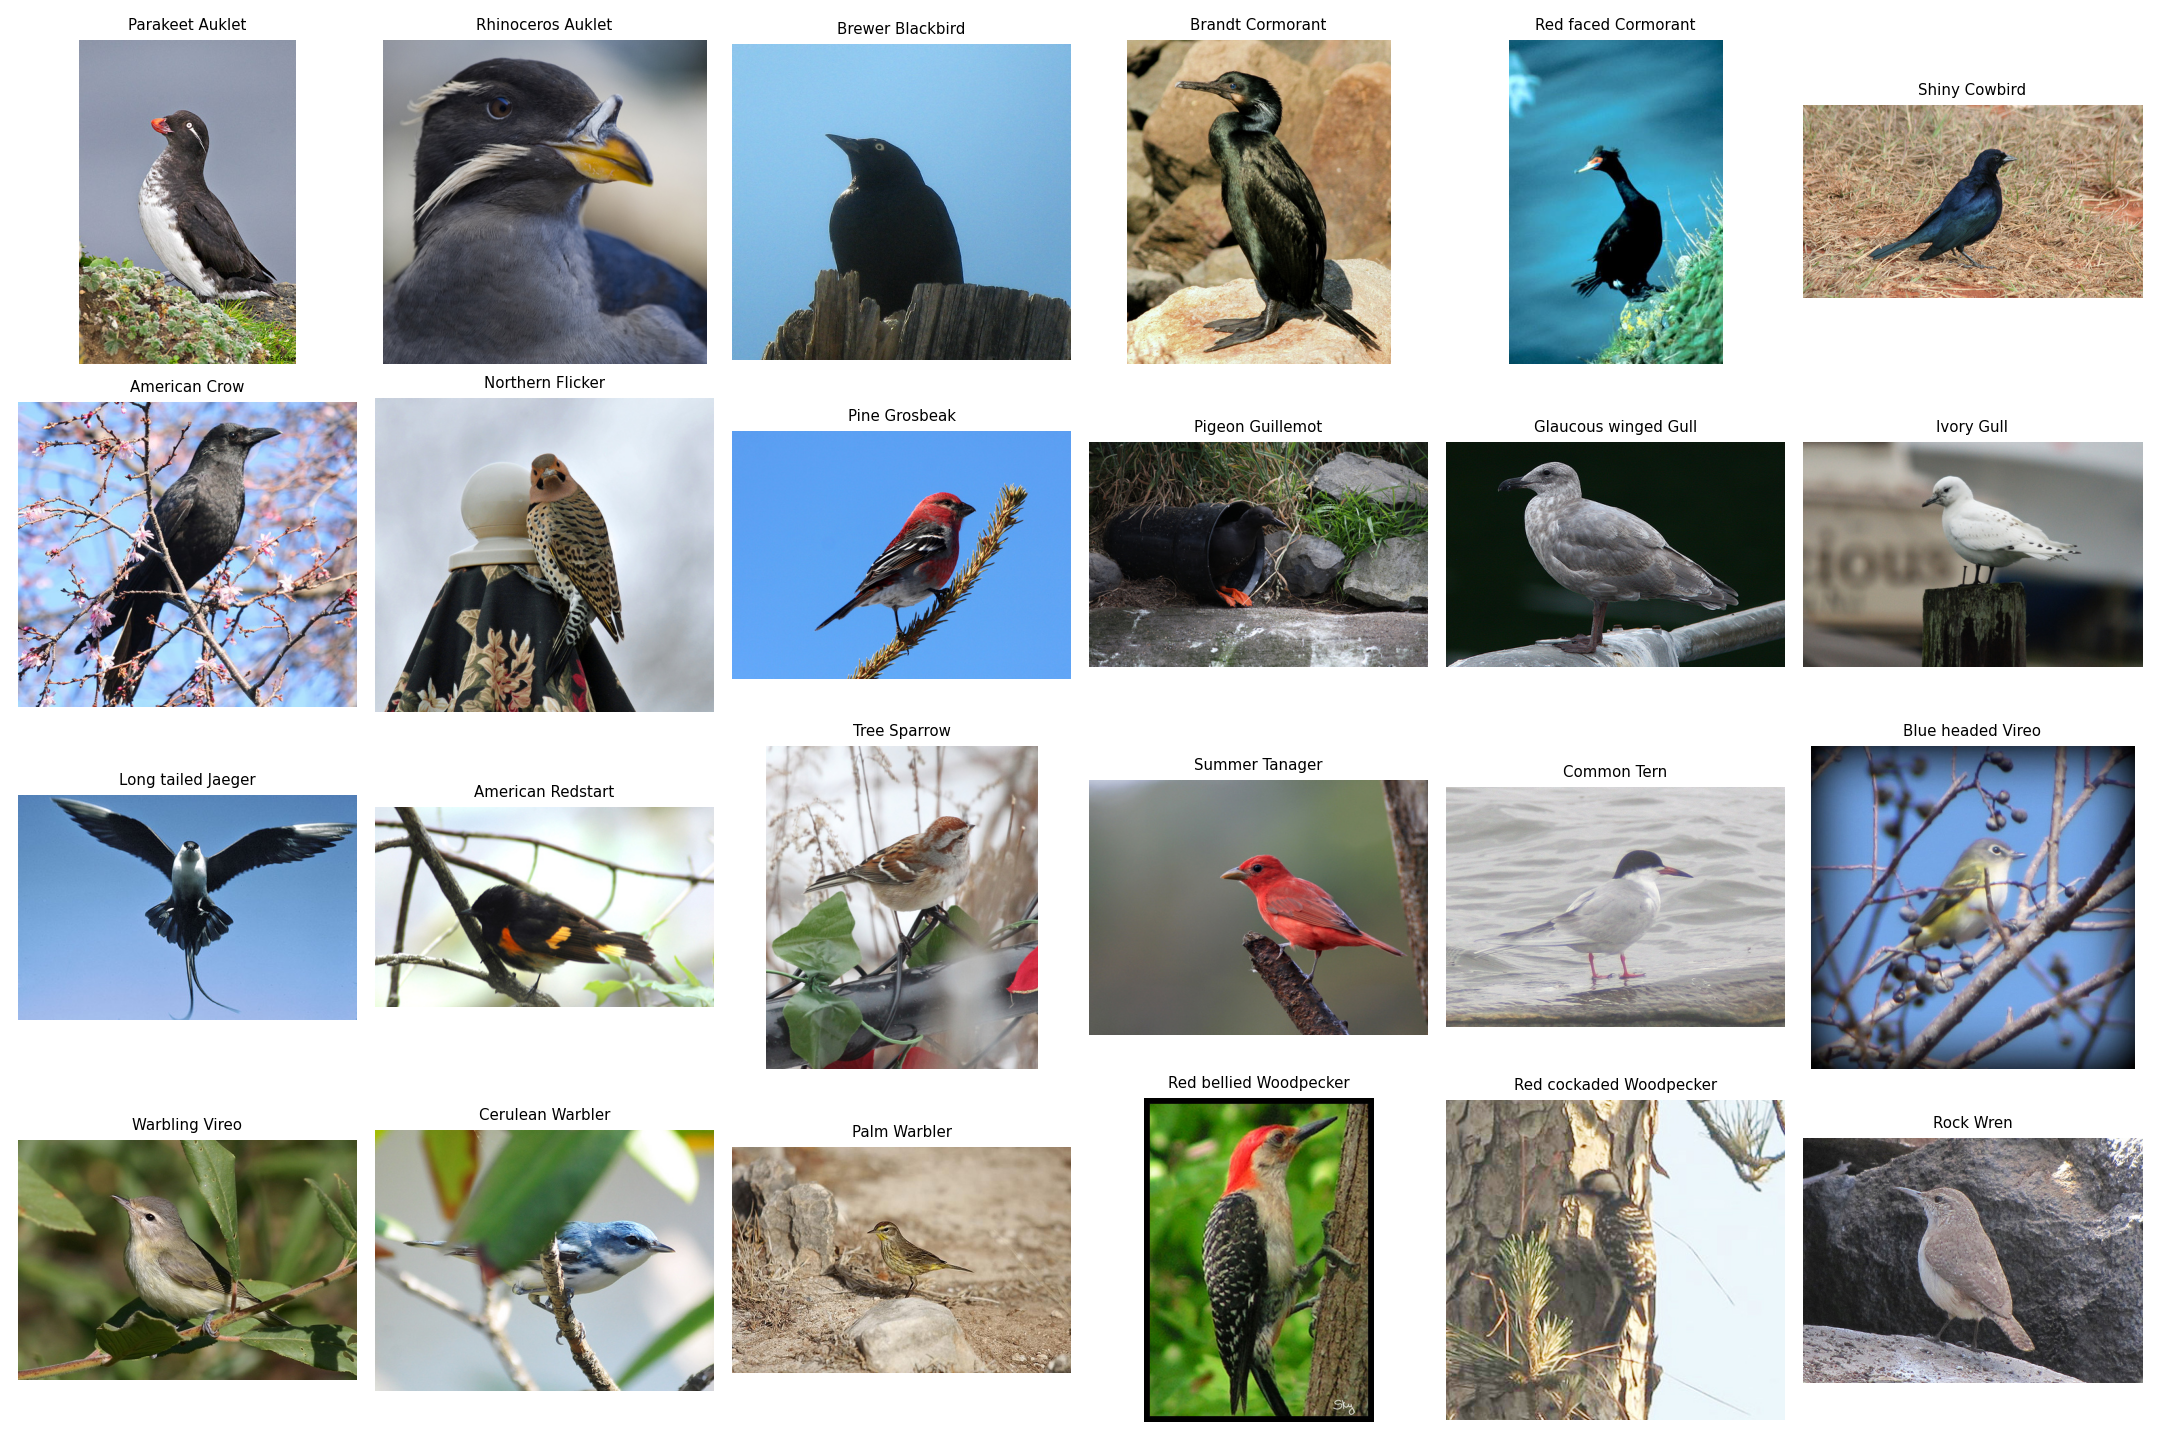
\includegraphics[width=0.85\linewidth]{eda_sample_grid.png}
\caption{Random sample of training images with their species names.}
\label{fig:samples}
\end{figure}

\subsection{Data splits}

The dataset only comes with a train set (5,994 images) and a test set (5,794 images), so there is no validation set. If we chose our hyperparameters by looking at the test accuracy, the test number would be too optimistic. So we took 3 images per class (600 in total) out of the train set and used them as validation. We did the split per class, because with only $\sim$30 images per species a normal random split could leave some species with no validation images at all. The indices are saved in \code{configs/splits/val\_indices.json} so that all of us used exactly the same split. The final split is in Table~\ref{tab:splits}.

\begin{table}[H]
\centering
\small
\begin{tabular}{l r l}
\toprule
\textbf{Split} & \textbf{Images} & \textbf{Used for} \\
\midrule
Train & 5,389 & training (5,994 $-$ 600 val $-$ 5 duplicates) \\
Validation & 600 & choosing models and hyperparameters \\
Test & 5,794 & final evaluation only \\
\bottomrule
\end{tabular}
\caption{Data splits used in all experiments.}
\label{tab:splits}
\end{table}

\subsection{Findings and the decisions we made}

\paragraph{Class balance.} The train set is almost perfectly balanced (26--27 images per class, imbalance ratio 1.04), but the test set is not (11--30 images per class, ratio 2.73), as can be seen in Figure~\ref{fig:classdist}. Because of this we did not use class weights, but we report \textbf{macro F1} next to accuracy, since macro F1 gives every species the same weight.

\begin{figure}[H]
\centering
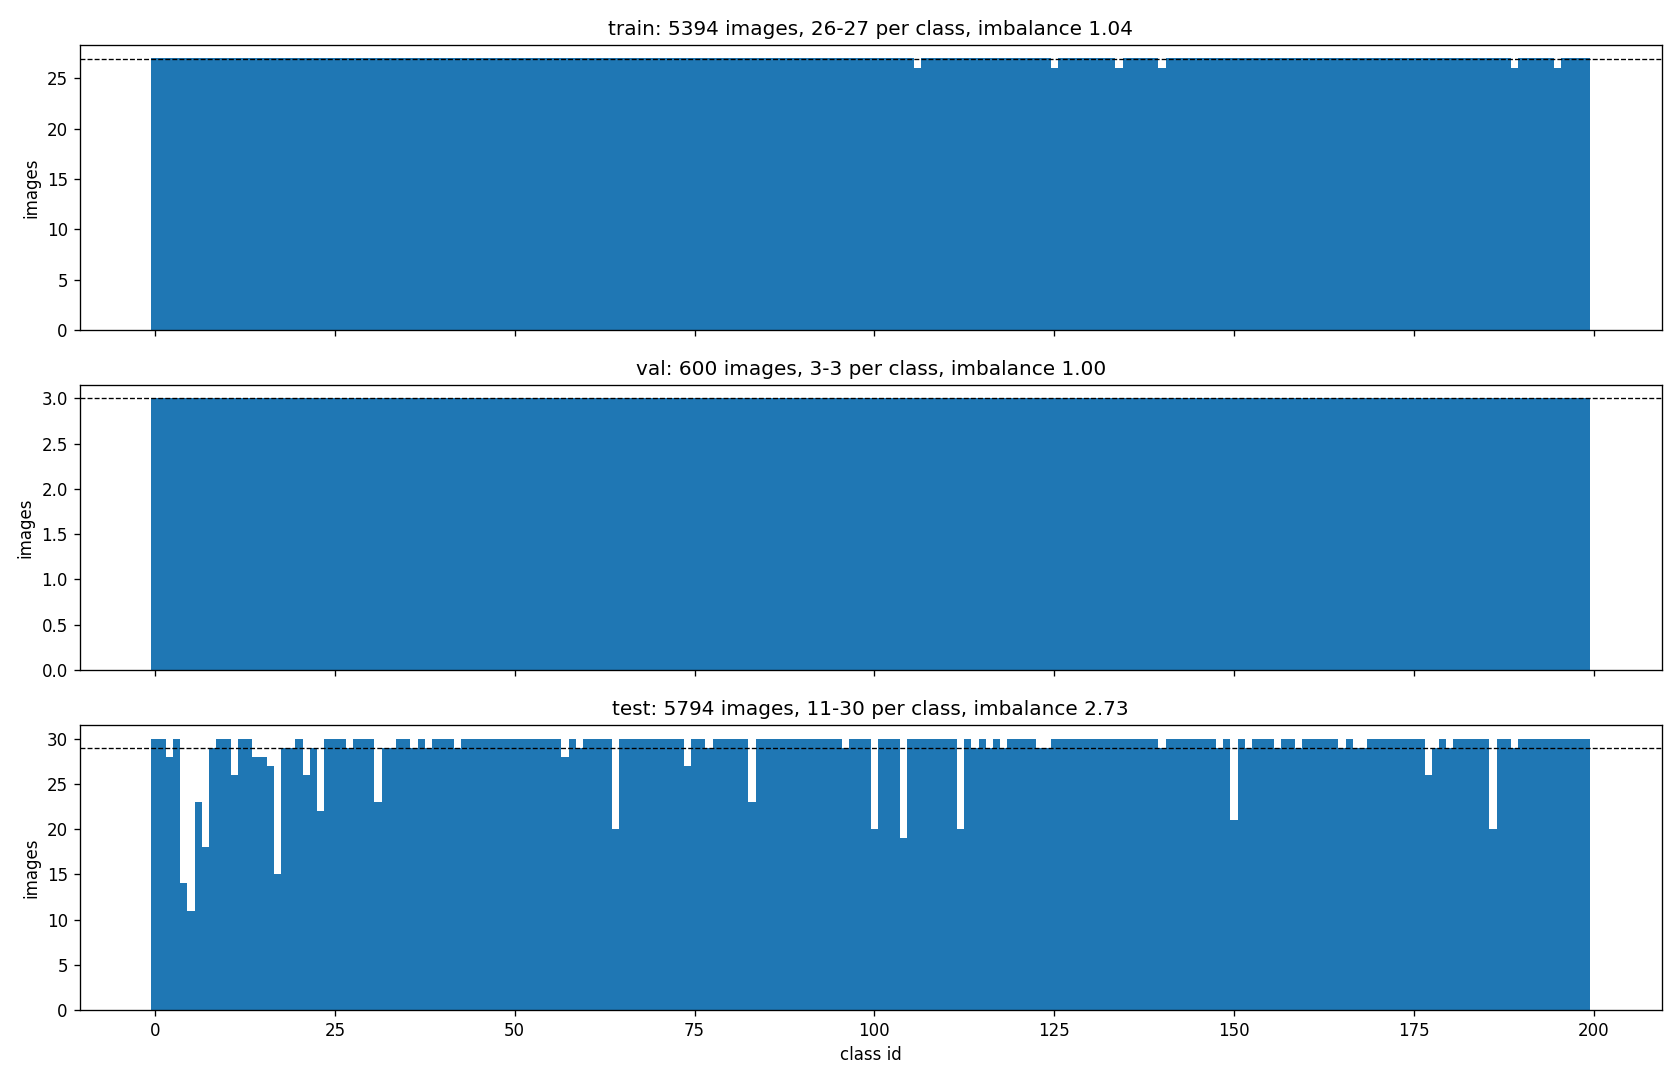
\includegraphics[width=0.8\linewidth]{eda_class_distribution.png}
\caption{Number of images per class in the train, validation and test splits.}
\label{fig:classdist}
\end{figure}

\paragraph{Image size and color mode.} Almost all images have a longest side of 500\,px (median $500\times375$), with aspect ratios between 0.38 and 3.6 (Figure~\ref{fig:imgstats}). Only 148 images have a side smaller than 224\,px, so resizing to 224 does not lose much. We found 8 grayscale images and no corrupted files, so we simply convert everything to RGB.

\begin{figure}[H]
\centering
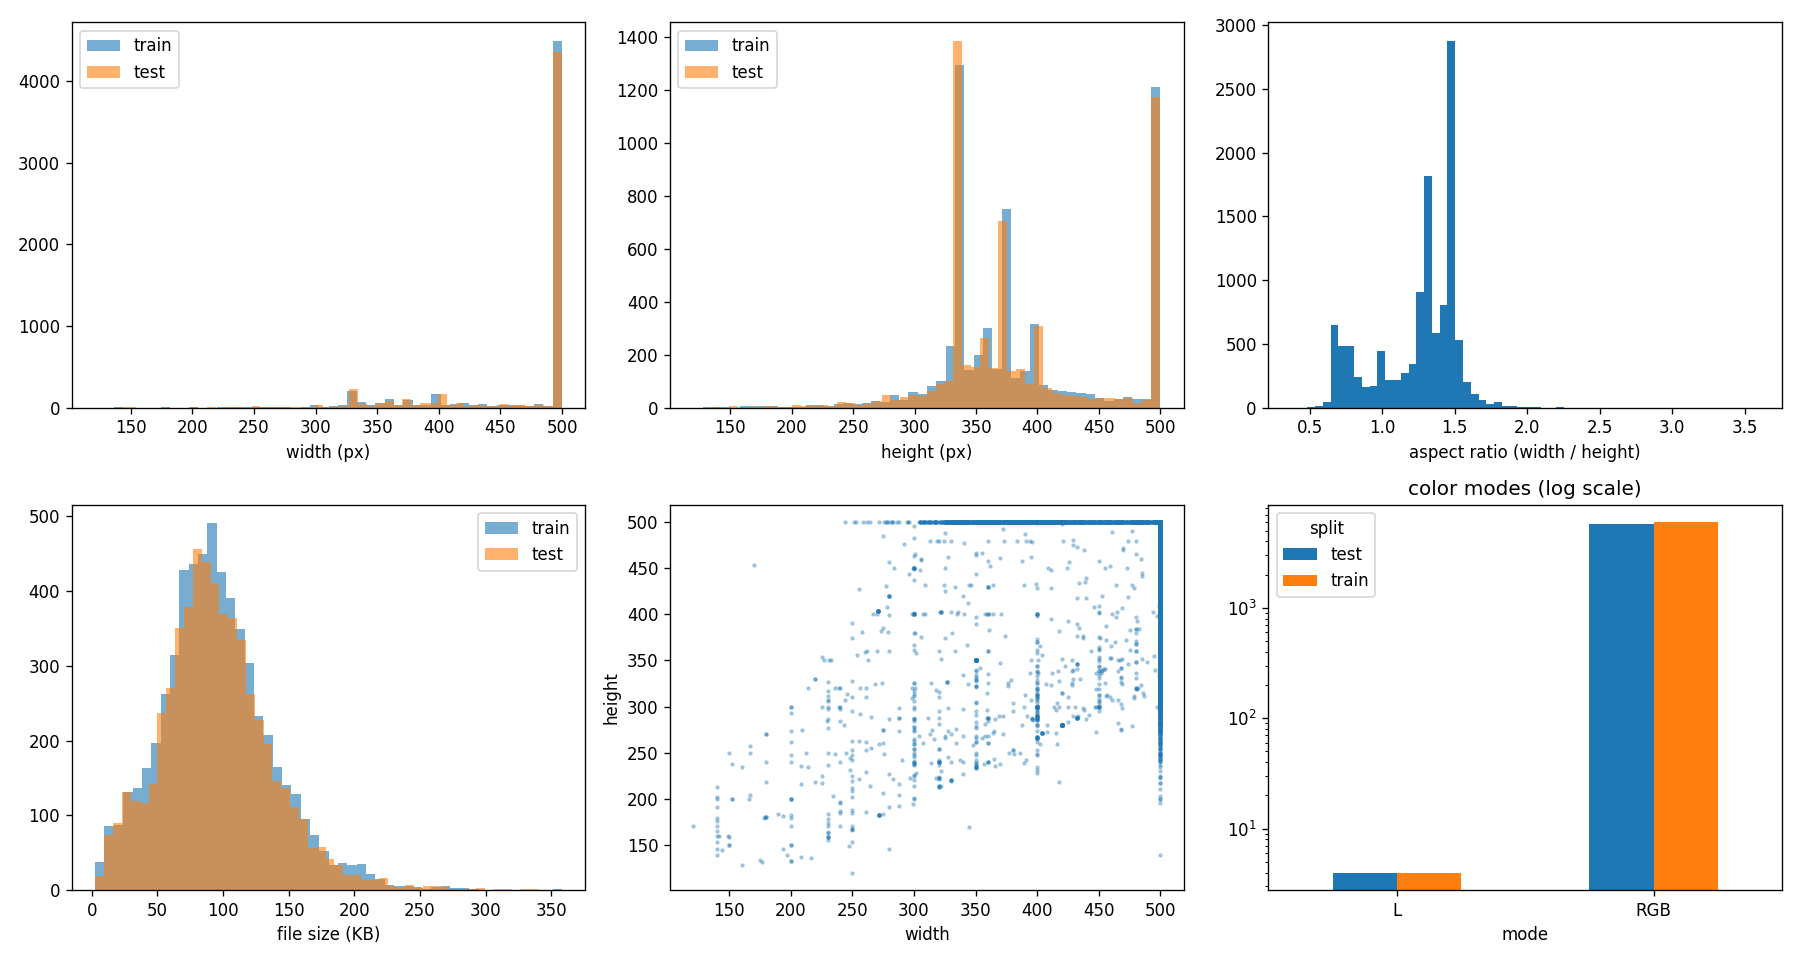
\includegraphics[width=0.85\linewidth]{eda_image_stats.png}
\caption{Image width, height, aspect ratio and file size distributions.}
\label{fig:imgstats}
\end{figure}

\paragraph{Duplicates.} We used perceptual hashing to look for duplicate images. pHash (distance $\le 4$) gave 8 candidate pairs, but when we looked at them, 3 of them were actually different birds on a plain sky or snow background. So we added a second check with dHash: the real duplicates differed by 0--1 bits and the false matches by 15--17 bits. In the end we had 3 train--train pairs and \textbf{2 train--test pairs} (Figure~\ref{fig:dups}). The train--test duplicates are a problem because the model would see test images during training, so we removed 5 images from the train set.

\paragraph{Channel statistics.} The mean of our train images is $(0.486, 0.501, 0.433)$ compared to ImageNet's $(0.485, 0.456, 0.406)$, so CUB is a bit greener and bluer, which makes sense with all the trees, sky and water (Figure~\ref{fig:channels}). We use the ImageNet values for pretrained models because they were trained with them, and the CUB values for the scratch CNN.

\begin{figure}[H]
\centering
\begin{subfigure}[b]{0.3\linewidth}
  \centering
  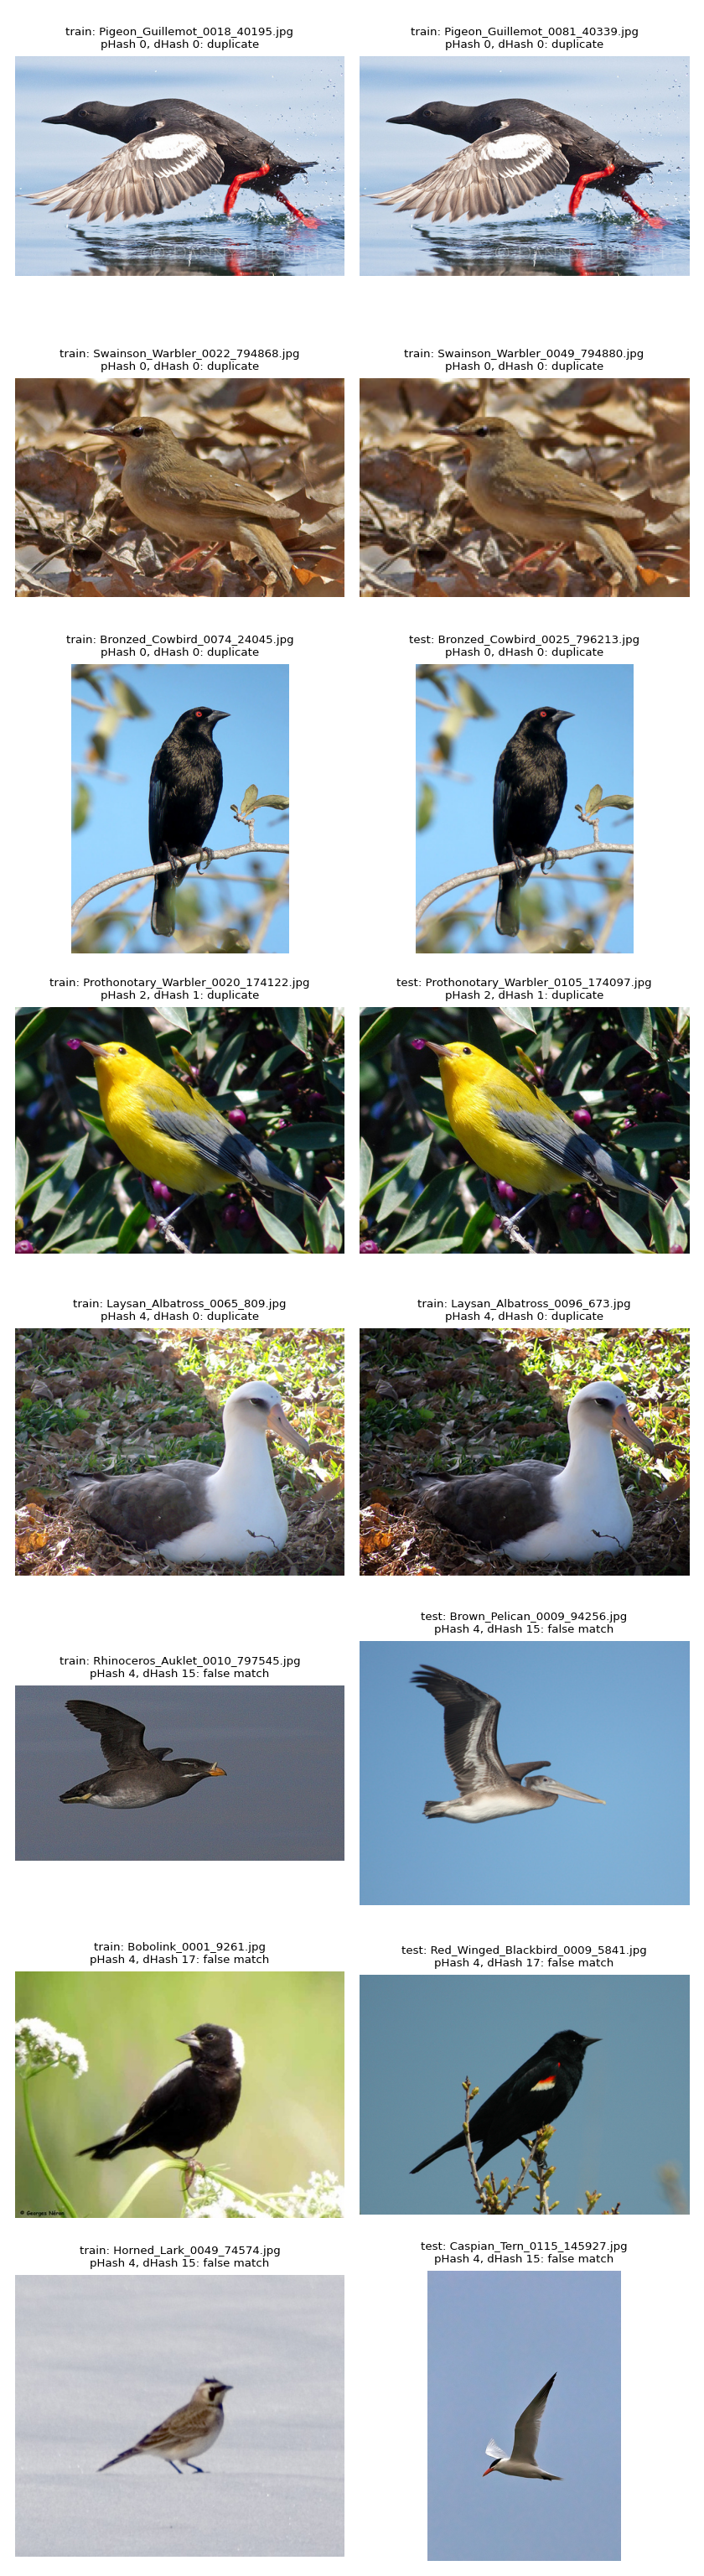
\includegraphics[height=8cm]{eda_duplicates.png}
  \caption{Duplicate pairs}
  \label{fig:dups}
\end{subfigure}
\hfill
\begin{subfigure}[b]{0.66\linewidth}
  \centering
  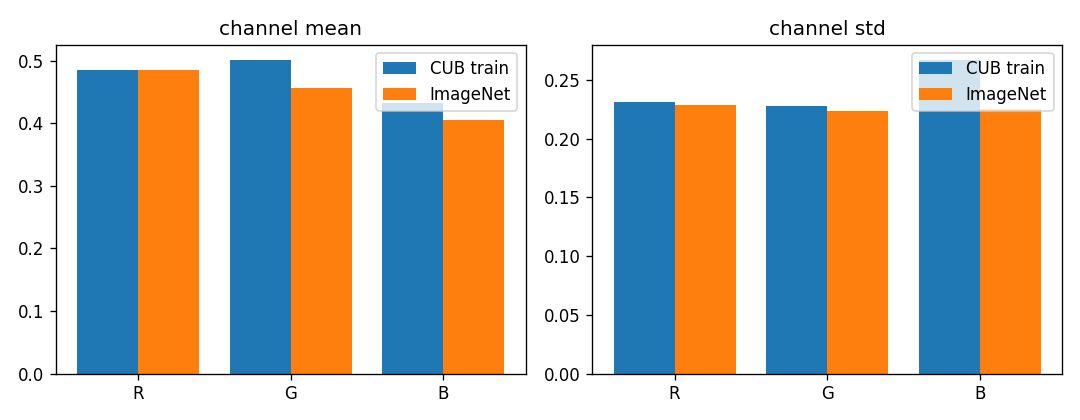
\includegraphics[width=\linewidth]{eda_channel_stats.png}
  \caption{Per-channel mean and std, CUB vs ImageNet}
  \label{fig:channels}
\end{subfigure}
\caption{Duplicate images found with pHash + dHash (left) and channel statistics (right).}
\end{figure}

\paragraph{Captions.} Even though captions are not used until Milestone 2, we analysed them now. Every image has exactly 10 captions, with an average length of 15.3 words and 95\% of them under 24 words (Figure~\ref{fig:captions}). About 100 captions had a broken Unicode replacement character in place of every space (e.g.\ ``this??bird??has''), and there were also many \texttt{/}, \texttt{;} and \texttt{\&} symbols. We wrote \code{clean\_caption()} to fix these. After cleaning, the vocabulary went from 6,690 to 4,076 words, and only 1,243 words appear at least 5 times. Most of the rare words are typos (e.g.\ ``abdomin'', ``ablack''), so in Milestone 2 we plan to keep words with frequency $\ge 5$ and map the rest to \code{<unk>}.

\begin{figure}[H]
\centering
\begin{subfigure}[b]{0.62\linewidth}
  \centering
  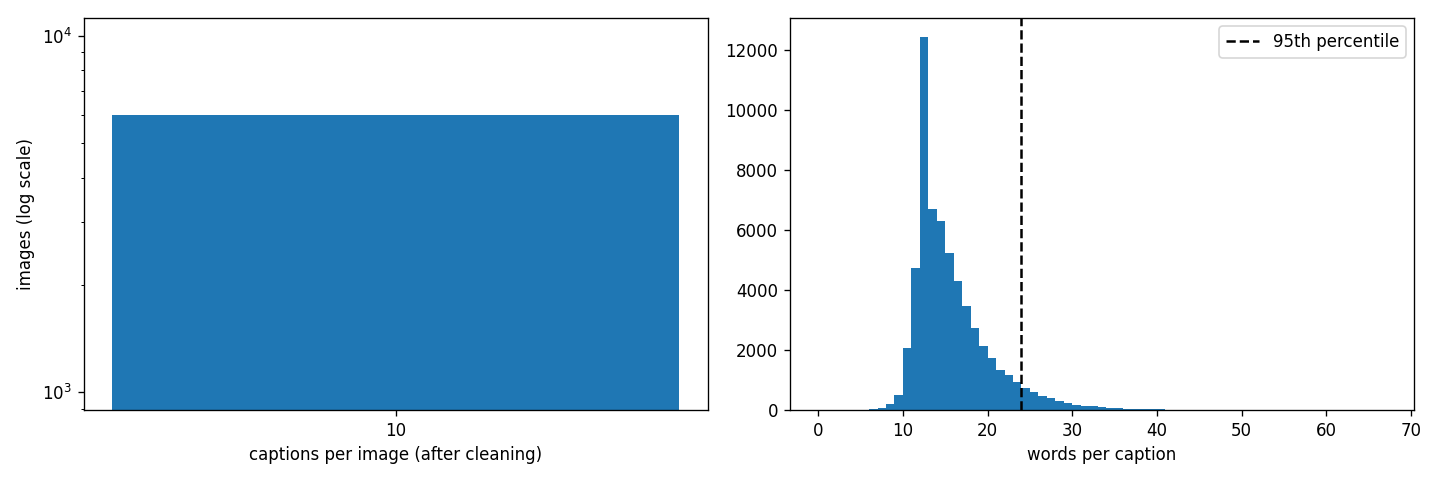
\includegraphics[width=\linewidth]{eda_caption_stats.png}
  \caption{Caption length and captions per image}
\end{subfigure}
\hfill
\begin{subfigure}[b]{0.34\linewidth}
  \centering
  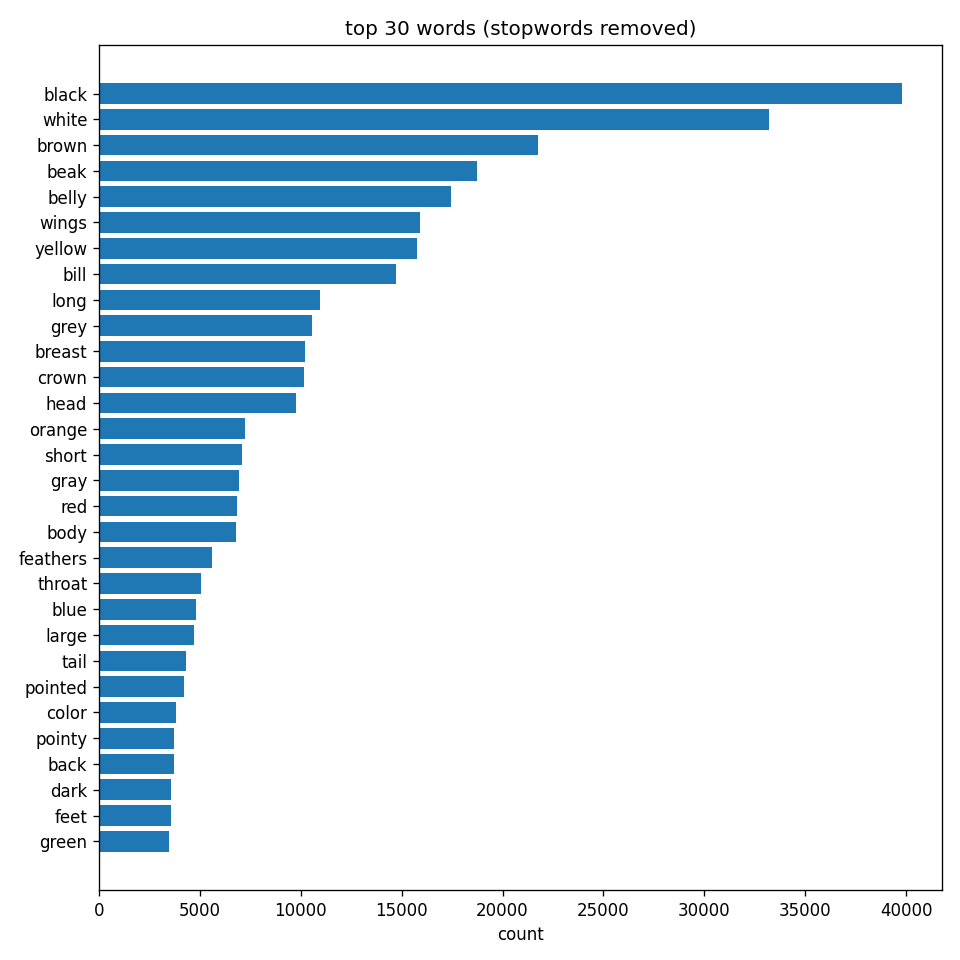
\includegraphics[width=\linewidth]{eda_top_words.png}
  \caption{Most frequent words}
\end{subfigure}
\caption{Caption statistics.}
\label{fig:captions}
\end{figure}

\subsection{Preprocessing and augmentation}

For training we use \code{RandomResizedCrop(224)} keeping 50--100\% of the image, horizontal flips, rotation up to $\pm10^\circ$, and mild color jitter (brightness, contrast and saturation 0.2). We kept the hue jitter very small (0.02) because color is often what separates two species, for example the Summer Tanager and the Scarlet Tanager. We also did not use vertical flips since birds are not upside down in real photos. For validation and test we resize to 256 and take a center crop of 224. Figure~\ref{fig:aug} shows some examples.

\begin{figure}[H]
\centering
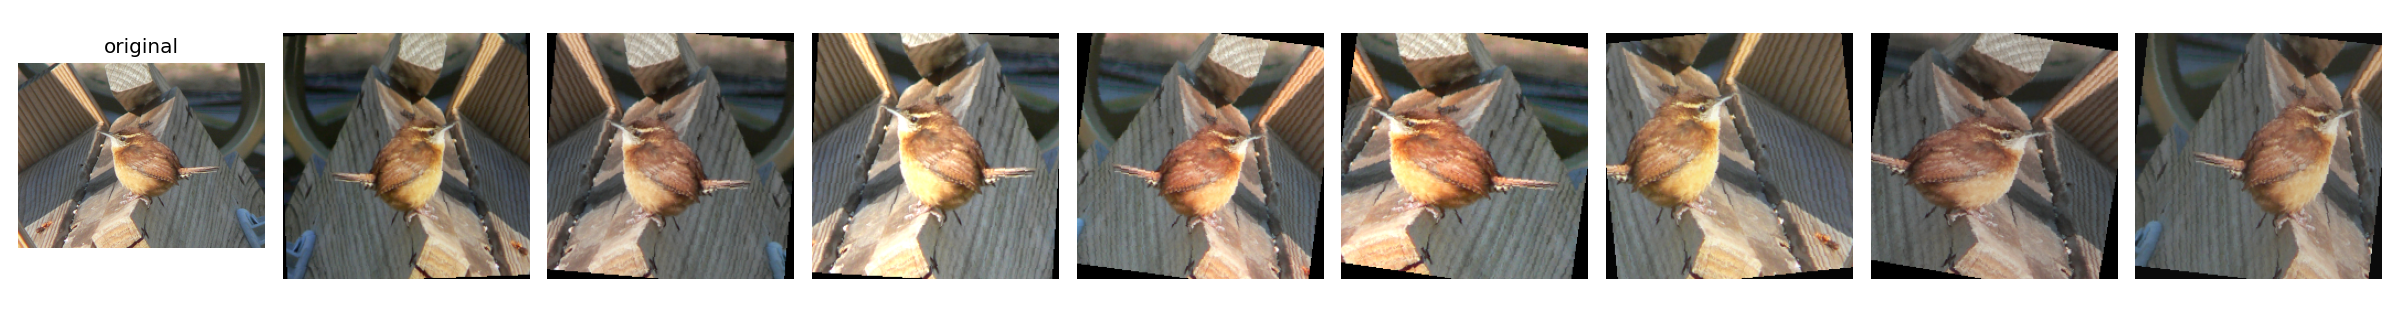
\includegraphics[width=\linewidth]{eda_augmentation_preview.png}
\caption{One training image with 8 random augmentations.}
\label{fig:aug}
\end{figure}

% =====================================================
\section{Models}

All encoders share the same interface: \code{forward\_features()} returns the spatial feature map, \code{forward()} returns the pooled vector, and \code{get\_gradcam\_layer()} returns the last convolutional layer. The classifier is just the encoder followed by dropout (0.3) and one linear layer with 200 outputs. This made it easy to switch between models without changing the training code.

\subsection{CNN from scratch}

Our baseline is a simple VGG-style network with 5 blocks, each made of two Conv3$\times$3--BatchNorm--ReLU layers followed by a 2$\times$2 max pool (Table~\ref{tab:scratch}). At the end we use global average pooling instead of flattening, so the last layer is $512\to200$ instead of $25{,}088\to200$, which gives far fewer parameters and less overfitting. The total is 4.82M parameters.

\begin{table}[H]
\centering
\small
\begin{tabular}{c c c}
\toprule
\textbf{Block} & \textbf{Channels} & \textbf{Output size} \\
\midrule
1 & $3 \to 32$    & $112\times112$ \\
2 & $32 \to 64$   & $56\times56$ \\
3 & $64 \to 128$  & $28\times28$ \\
4 & $128 \to 256$ & $14\times14$ \\
5 & $256 \to 512$ & $7\times7$ \\
GAP + dropout + linear & $512 \to 200$ & $1\times1$ \\
\bottomrule
\end{tabular}
\caption{Architecture of the scratch CNN for a $224\times224$ input.}
\label{tab:scratch}
\end{table}

\subsection{Pretrained ResNet-50}

For transfer learning we used ResNet-50~\cite{he2016resnet} with the torchvision \code{IMAGENET1K\_V2} weights, after removing its pooling and 1000-class layer. It gives a $2048\times7\times7$ feature map. We tried it in two ways:
\begin{itemize}
  \item \textbf{Frozen:} the backbone is locked and only the last linear layer is trained (0.41M trainable parameters out of 23.9M). We also had to keep the backbone in eval mode, because otherwise BatchNorm keeps updating its running statistics even when the weights are frozen.
  \item \textbf{Fine-tuned:} all layers are trained, with a small learning rate ($10^{-4}$) so the ImageNet features are adjusted rather than destroyed.
\end{itemize}

% =====================================================
\section{Training Setup}

All models were trained with the same function, \code{train\_model()}, using cross-entropy loss, AdamW~\cite{loshchilov2019adamw}, a cosine learning rate schedule~\cite{loshchilov2017sgdr}, batch size 32 and mixed precision on the GPU. We use early stopping on \emph{validation accuracy} and keep the checkpoint of the best epoch. We chose accuracy instead of loss because with so few images per class the validation loss could keep going down even after the accuracy stopped improving. All runs were done on a Kaggle T4 GPU, since one epoch on a laptop CPU took about 16 minutes. Every run is logged to MLflow with its config, per-epoch metrics, curves and checkpoint.

\begin{table}[H]
\centering
\small
\begin{tabular}{l c c c c}
\toprule
\textbf{Model} & \textbf{lr} & \textbf{Max epochs} & \textbf{Patience} & \textbf{Normalization} \\
\midrule
Scratch CNN        & $3\times10^{-4}$ & 40 & 10 & CUB \\
ResNet-50 frozen   & $1\times10^{-3}$ & 15 & 5  & ImageNet \\
ResNet-50 fine-tuned & $1\times10^{-4}$ & 20 & 5  & ImageNet \\
\bottomrule
\end{tabular}
\caption{Training settings. Weight decay is $10^{-4}$ for all models.}
\label{tab:settings}
\end{table}

% =====================================================
\section{Results}

\subsection{Scratch CNN vs transfer learning}

Table~\ref{tab:results} summarizes the results on the test set and Figure~\ref{fig:curves} shows the training curves.

\begin{table}[H]
\centering
\small
\begin{tabular}{l r c c c c r}
\toprule
\textbf{Model} & \textbf{Trainable} & \textbf{Train acc} & \textbf{Best val acc} & \textbf{Test acc} & \textbf{Macro F1} & \textbf{Time} \\
\midrule
Scratch CNN          & 4.82M & 47.3\% & 38.3\% (ep.\ 39) & 40.2\% & 38.8\% & -- \\
ResNet-50 frozen     & 0.41M & 81.9\% & 61.0\% (ep.\ 11) & 64.3\% & 64.0\% & 9.6 min \\
\textbf{ResNet-50 fine-tuned} & 23.9M & 99.1\% & \textbf{82.0\%} (ep.\ 16) & \textbf{82.9\%} & \textbf{82.9\%} & 13.3 min \\
ResNet-50 tuned      & 23.9M & 99.4\% & 81.3\% (ep.\ 11) & 81.8\% & 81.8\% & 10.7 min \\
\bottomrule
\end{tabular}
\caption{Results on the test set (5,794 images). Random guessing would give 0.5\%.}
\label{tab:results}
\end{table}

\begin{figure}[H]
\centering
\begin{subfigure}{\linewidth}
  \centering
  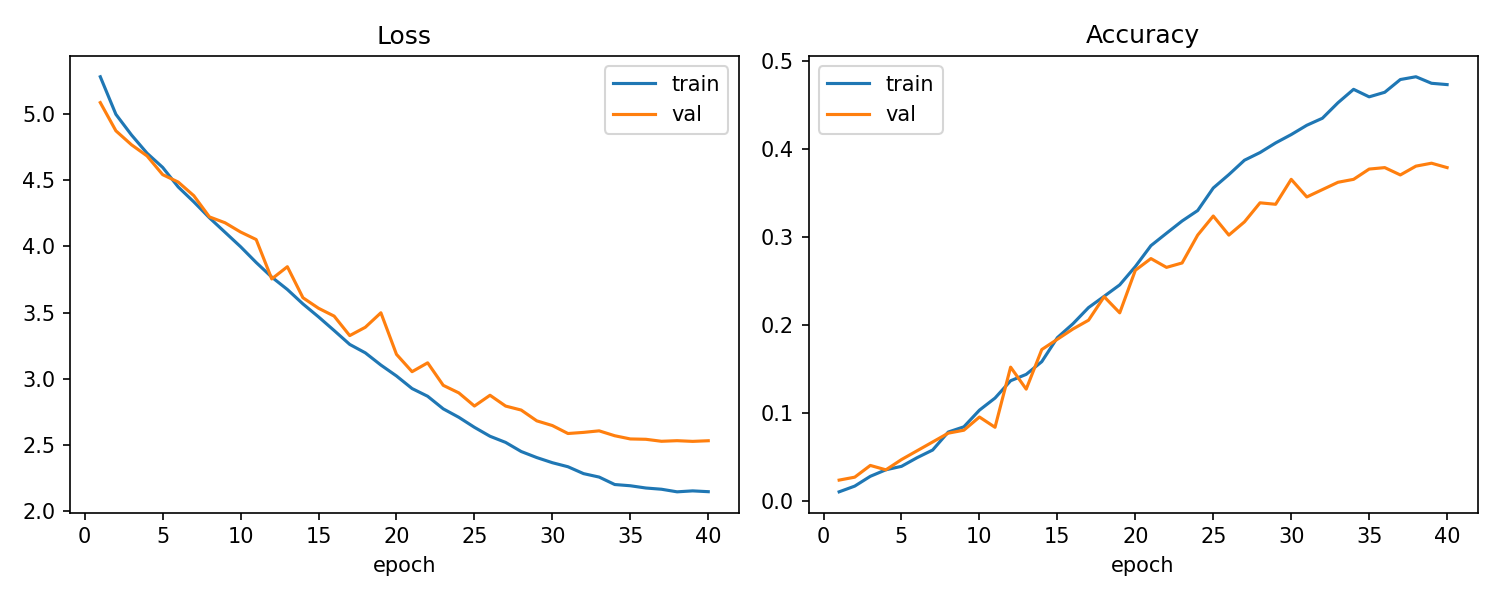
\includegraphics[width=0.85\linewidth]{scratch_baseline_curves.png}
  \caption{Scratch CNN}
\end{subfigure}

\begin{subfigure}{\linewidth}
  \centering
  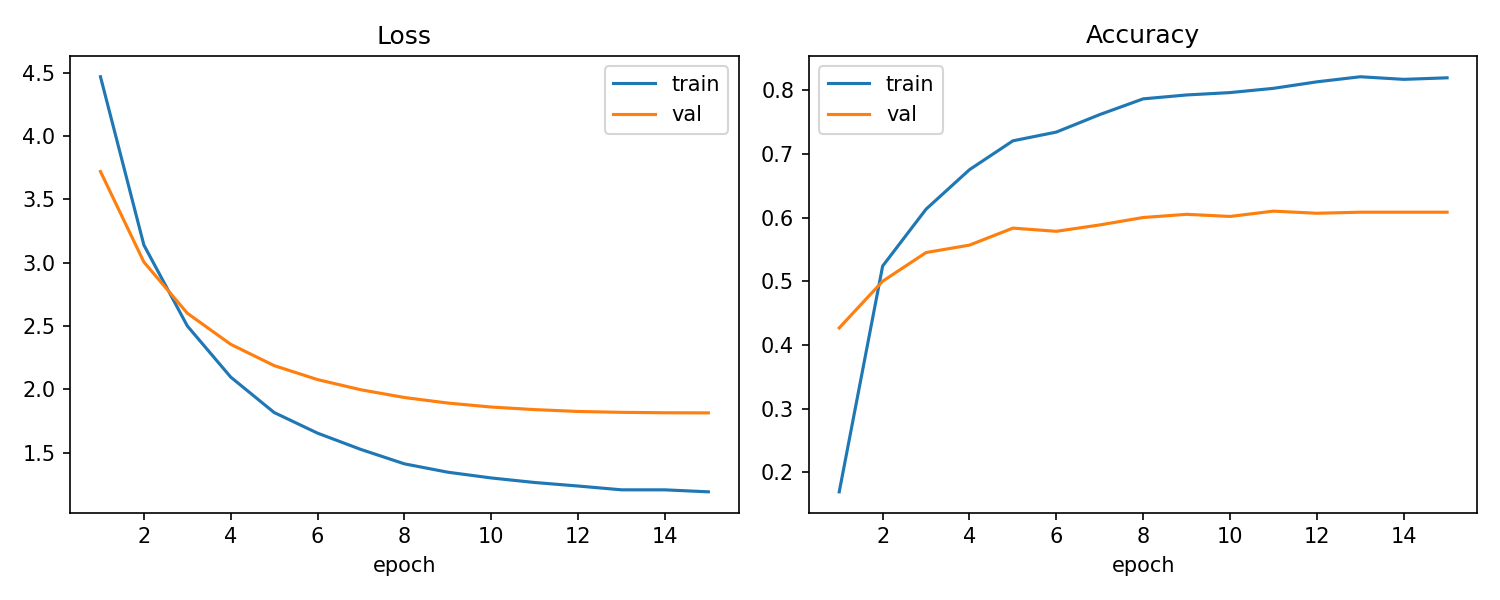
\includegraphics[width=0.85\linewidth]{cls_resnet50_frozen.png}
  \caption{ResNet-50, frozen backbone}
\end{subfigure}

\begin{subfigure}{\linewidth}
  \centering
  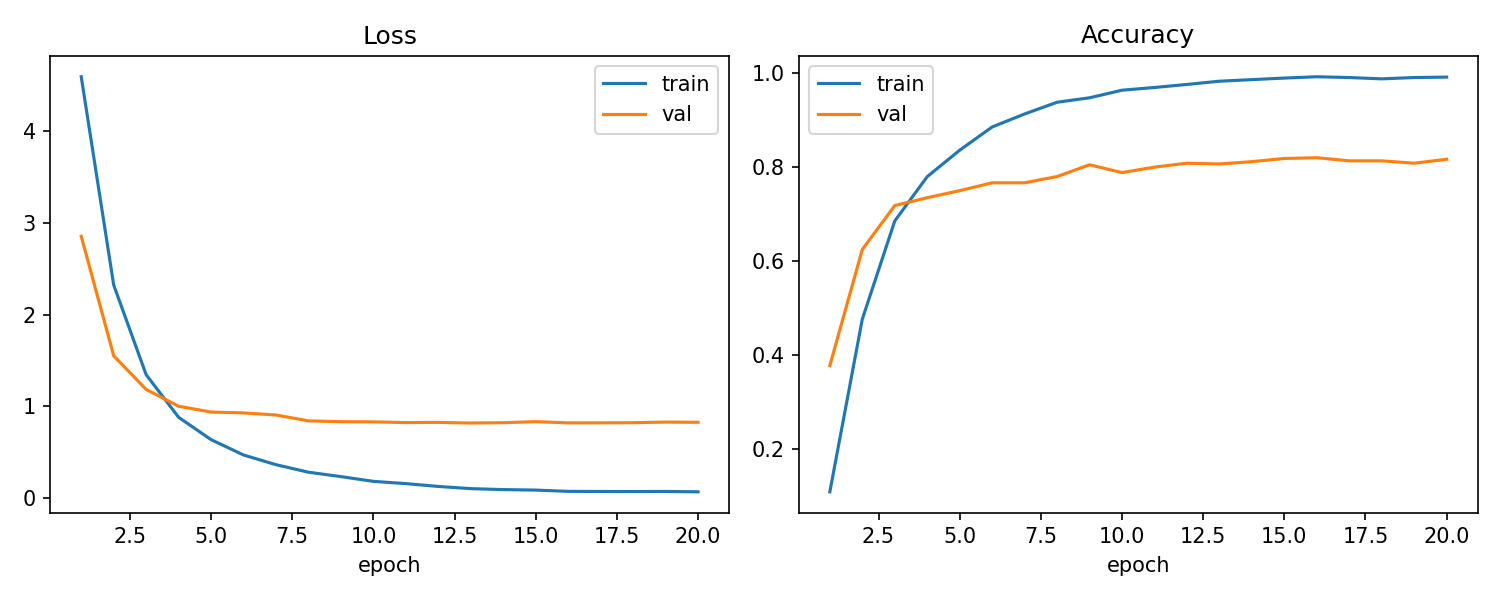
\includegraphics[width=0.85\linewidth]{cls_resnet50_finetune.png}
  \caption{ResNet-50, fine-tuned}
\end{subfigure}
\caption{Training and validation loss and accuracy for the three models.}
\label{fig:curves}
\end{figure}

\paragraph{Scratch CNN (40.2\%).} This is about 80 times better than chance, but still low. With only $\sim$27 images per species and no prior knowledge, the network cannot really learn the small details that separate similar species. The gap between train (47.3\%) and validation (38.3\%) is only about 9 points, so the model is underfitting more than overfitting. Early stopping never triggered because the validation accuracy was still slowly going up at epoch 40, but by then the cosine schedule had brought the learning rate to almost zero. The top-5 accuracy was 72\%, so the right species is usually among the first guesses.

\paragraph{Frozen ResNet-50 (64.3\%).} Just by training one linear layer on top of ImageNet features we gained 24 points, which shows how much the pretrained features already help. The validation accuracy stopped improving after epoch 11, because a single linear layer on fixed features does not have enough capacity to go further.

\paragraph{Fine-tuned ResNet-50 (82.9\%).} Letting all the layers adapt to birds added another 18.6 points and more than doubled the scratch CNN. The training accuracy reached 99\% while validation stayed around 82\%, so the model basically memorized the training set. However, the validation loss did not go up, so this did not hurt generalization. Macro F1 is equal to accuracy, which means the model is not only doing well on species that have more test images.

\subsection{Hyperparameter tuning}

We tuned the learning rate and weight decay of the fine-tuned ResNet-50 with both grid search and random search. Each trial ran for 5 epochs with the same seed and used only the train and validation sets. The grid was $\text{lr}\in\{10^{-4}, 3\times10^{-4}\}\times\text{wd}\in\{10^{-4},10^{-3}\}$. For random search we sampled 4 points log-uniformly between the same limits, since sampling from the same 4 grid points would just be the grid in a different order~\cite{bergstra2012random}.

\begin{table}[H]
\centering
\small
\begin{tabular}{l c c c c r}
\toprule
\textbf{Method} & \textbf{Best lr} & \textbf{Best wd} & \textbf{Best val acc (5 ep.)} & \textbf{Trials} & \textbf{Time} \\
\midrule
Grid   & $3\times10^{-4}$    & $1\times10^{-4}$    & 79.5\% & 4 & 12.5 min \\
Random & $1.35\times10^{-4}$ & $1.67\times10^{-4}$ & 79.7\% & 4 & 12.6 min \\
\bottomrule
\end{tabular}
\caption{Grid search vs random search.}
\label{tab:tuning}
\end{table}

We then trained the best setting (from random search) for the full schedule. It got 81.3\% validation and 81.8\% test accuracy, which is actually \emph{a bit worse} than our default setting (82.0\% / 82.9\%). We think there are three reasons for this:
\begin{enumerate}
  \item The trials were only 5 epochs long, and the best setting after 5 epochs is not necessarily the best after 20.
  \item All the trials with lr between $1.35\times10^{-4}$ and $3\times10^{-4}$ ended between 78.2\% and 79.7\%. On 600 validation images, 1 point is only 6 images, so these differences are basically noise.
  \item Our default lr of $10^{-4}$ was already in the good range.
\end{enumerate}
Since we select models by validation accuracy and not test accuracy, we kept the untuned fine-tuned ResNet-50 as our final model. With only 2 hyperparameters and 4 trials, grid and random search performed the same; we expect random search to be more useful when there are more hyperparameters.

% =====================================================
\section{Error Analysis and Grad-CAM}

\subsection{Most confused species}

Using the confusion matrix on the test set, we listed the 5 species pairs that each model mixes up the most, counting mistakes in both directions (Table~\ref{tab:confused}).

\begin{table}[H]
\centering
\small
\begin{tabular}{c l l}
\toprule
\textbf{\#} & \textbf{Scratch CNN} & \textbf{ResNet-50 fine-tuned} \\
\midrule
1 & Eared Grebe $\leftrightarrow$ Horned Grebe (13) & Long-tailed Jaeger $\leftrightarrow$ Pomarine Jaeger (15) \\
2 & Arctic Tern $\leftrightarrow$ Common Tern (13) & Chuck-will's-widow $\rightarrow$ Whip-poor-will (14) \\
3 & Loggerhead Shrike $\leftrightarrow$ Great Grey Shrike (12) & Brandt's Cormorant $\leftrightarrow$ Pelagic Cormorant (14) \\
4 & Arctic Tern $\leftrightarrow$ Forster's Tern (12) & Acadian Flycatcher $\leftrightarrow$ Yellow-bellied Flycatcher (12) \\
5 & Blue-winged Warbler $\leftrightarrow$ Prothonotary Warbler (12) & Arctic Tern $\leftrightarrow$ Common Tern (12) \\
\bottomrule
\end{tabular}
\caption{The 5 most confused species pairs on the test set (number of mistakes).}
\label{tab:confused}
\end{table}

All of the ResNet-50 pairs are species from the same family that look almost identical, and that even bird watchers often separate by their song, so we consider these ``reasonable'' mistakes. Interestingly, the Chuck-will's-widow mistake only goes one way: the model labels both species as Whip-poor-will. The scratch CNN, on the other hand, also confuses species that only share a color, like the Blue-winged and Prothonotary Warblers, which are both yellow but otherwise look different. This suggests it relies on color more than on shape.

\subsection{Grad-CAM}

We implemented Grad-CAM~\cite{selvaraju2017gradcam} ourselves using PyTorch hooks. A forward hook on the last convolutional layer stores the feature maps $A^k$, and a hook on the output tensor stores their gradients when the class score $y^c$ is backpropagated. The weight of each channel is the average of its gradient, and the heatmap is
\begin{equation}
  \alpha_k^c = \frac{1}{Z}\sum_{i,j}\frac{\partial y^c}{\partial A^k_{ij}}, \qquad
  L^c_{\text{Grad-CAM}} = \mathrm{ReLU}\Big(\sum_k \alpha_k^c A^k\Big),
\end{equation}
which we then resize to $224\times224$ and normalize to $[0,1]$. One problem we ran into is that for the frozen ResNet-50 no gradient flows to \code{layer4} because none of its weights need gradients, so the hook never fired. We fixed this by setting \code{requires\_grad} on the input image.

\begin{figure}[H]
\centering
\begin{subfigure}[b]{0.49\linewidth}
  \centering
  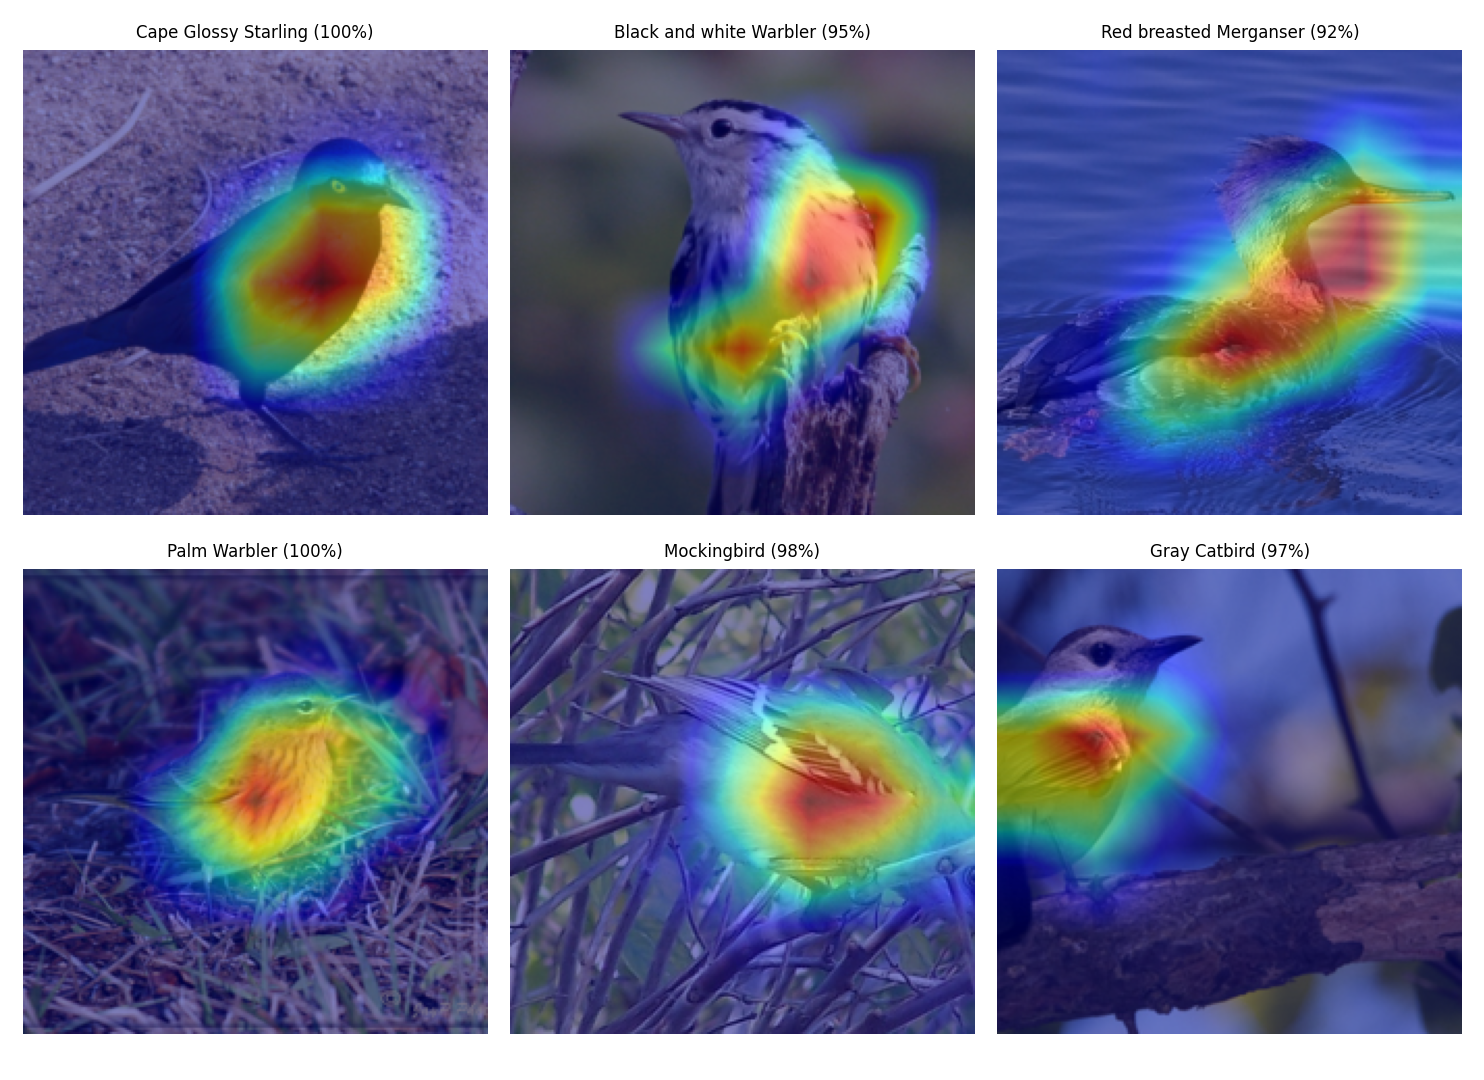
\includegraphics[width=\linewidth]{gradcam_resnet50_correct.png}
  \caption{ResNet-50, correct predictions}
\end{subfigure}
\hfill
\begin{subfigure}[b]{0.49\linewidth}
  \centering
  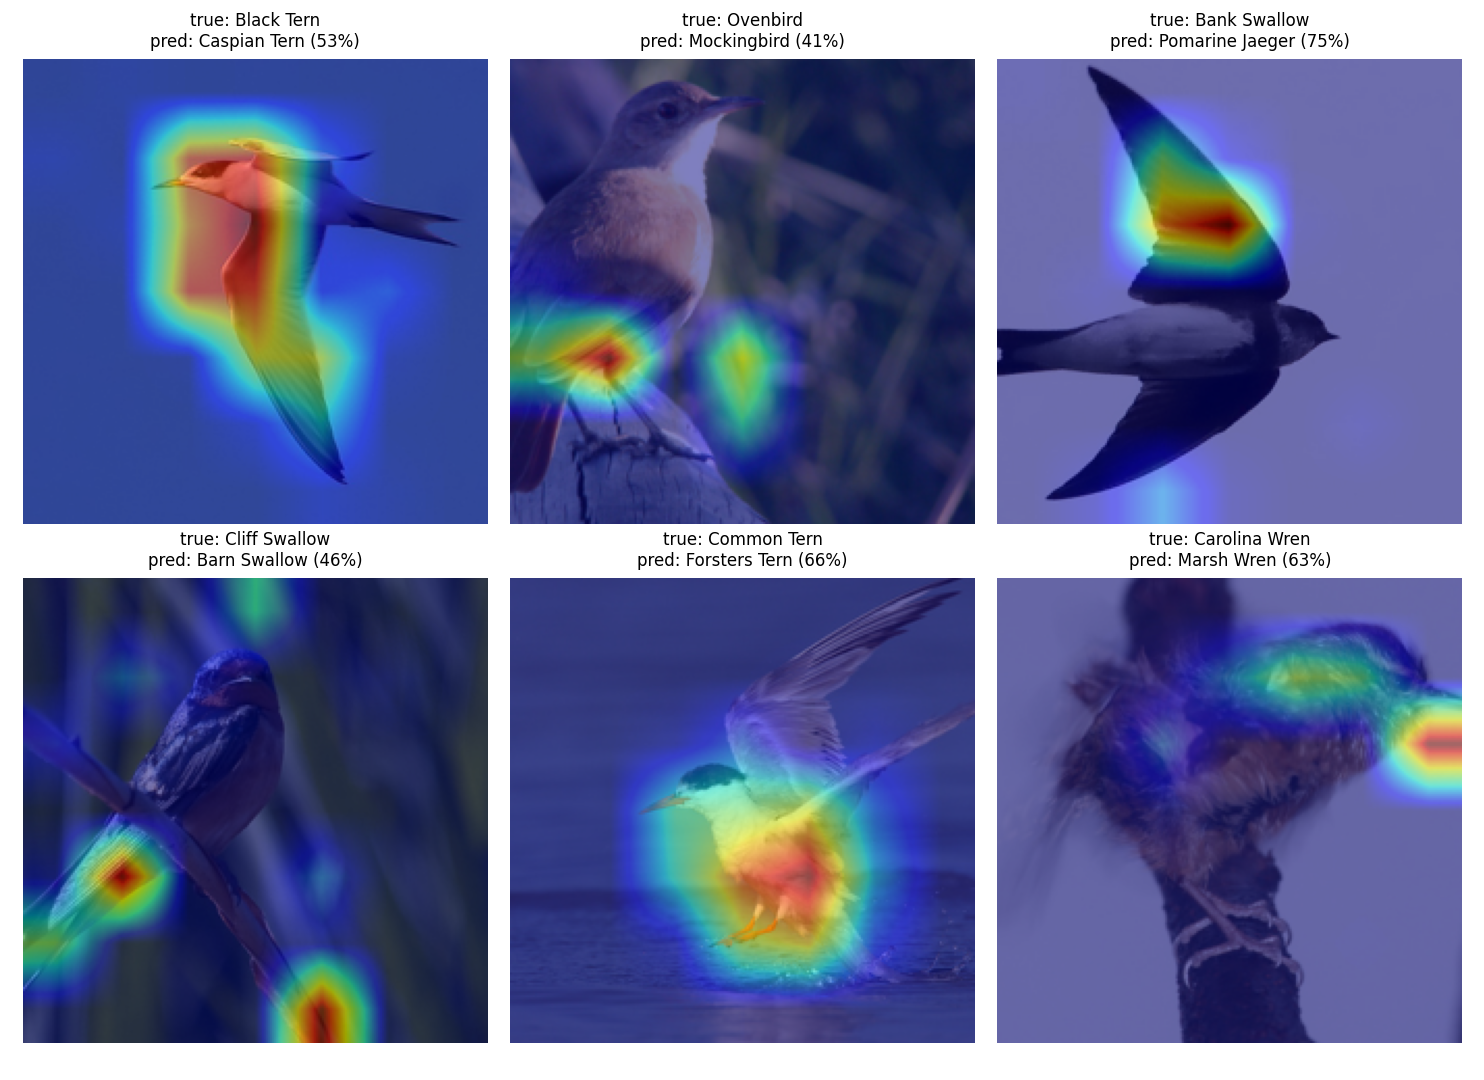
\includegraphics[width=\linewidth]{gradcam_resnet50_wrong.png}
  \caption{ResNet-50, wrong predictions}
\end{subfigure}

\vspace{4pt}
\begin{subfigure}[b]{0.49\linewidth}
  \centering
  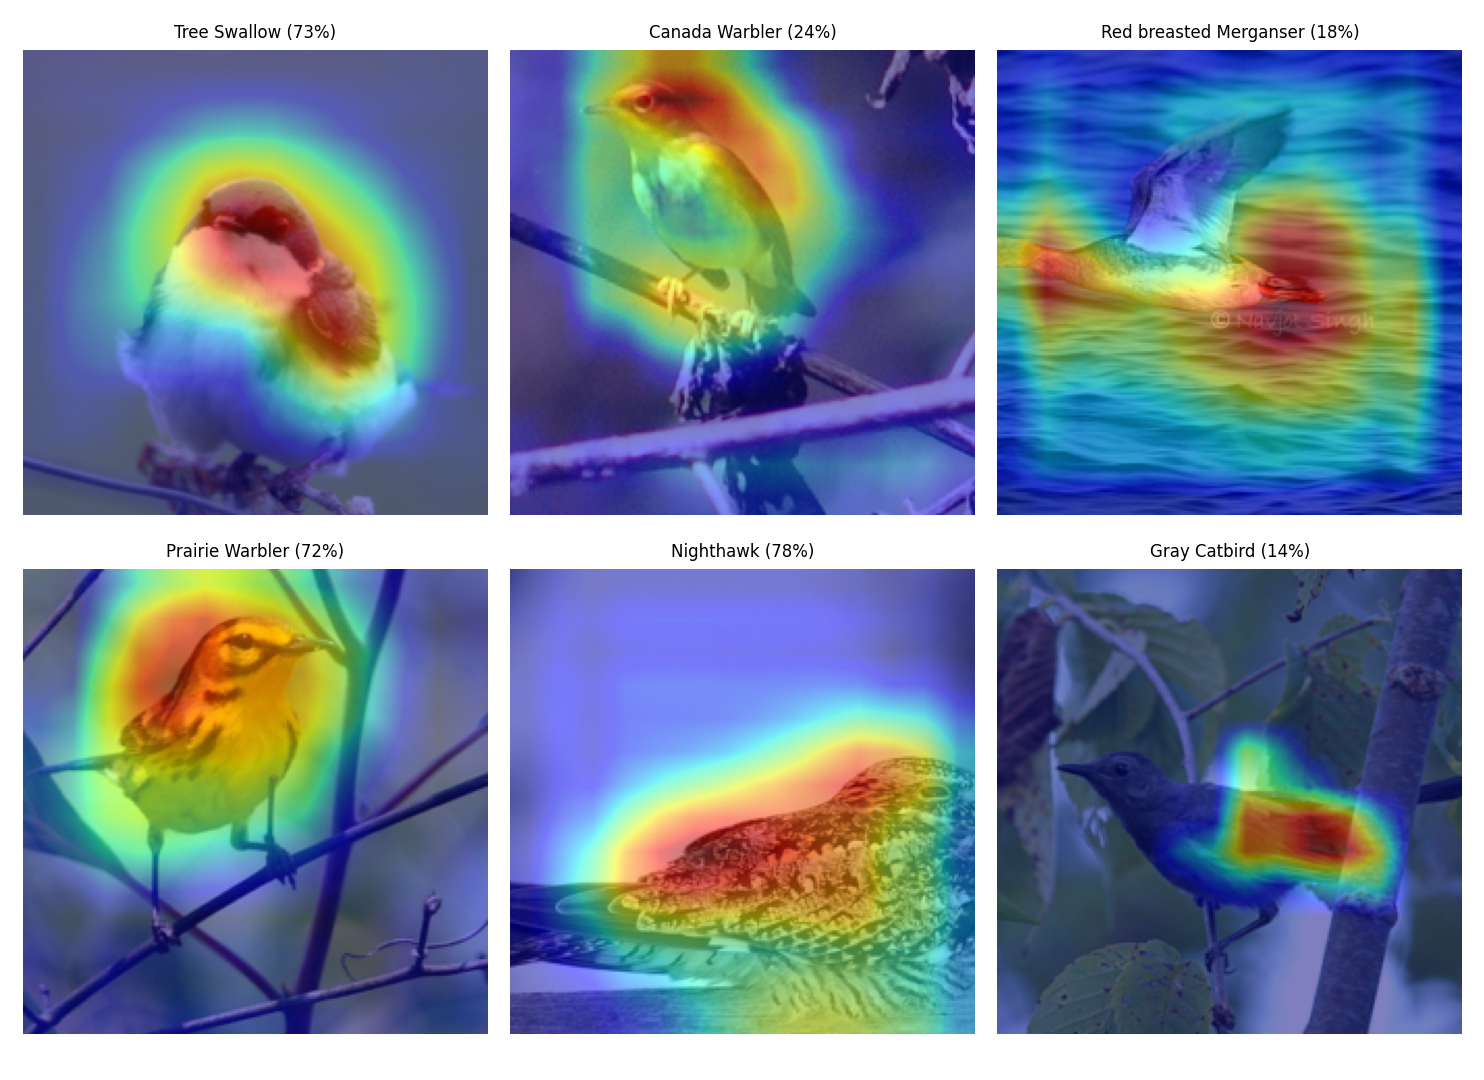
\includegraphics[width=\linewidth]{gradcam_scratch_correct.png}
  \caption{Scratch CNN, correct predictions}
\end{subfigure}
\hfill
\begin{subfigure}[b]{0.49\linewidth}
  \centering
  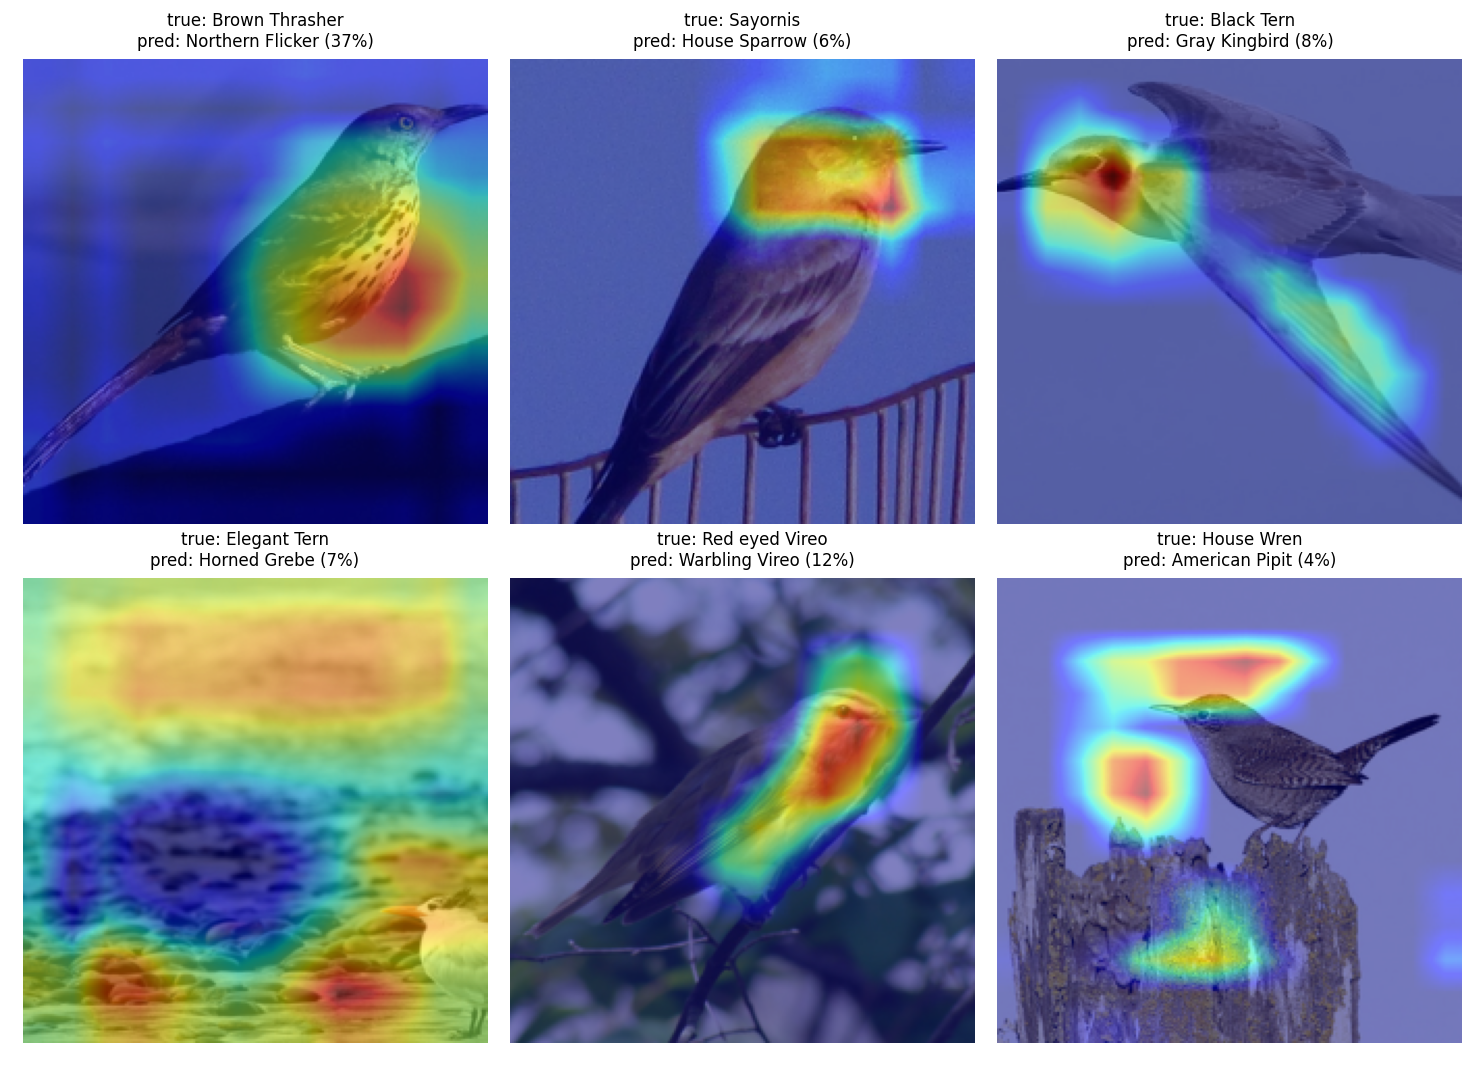
\includegraphics[width=\linewidth]{gradcam_scratch_wrong.png}
  \caption{Scratch CNN, wrong predictions}
\end{subfigure}
\caption{Grad-CAM heatmaps on random correct and wrong test predictions.}
\label{fig:gradcam}
\end{figure}

\begin{figure}[H]
\centering
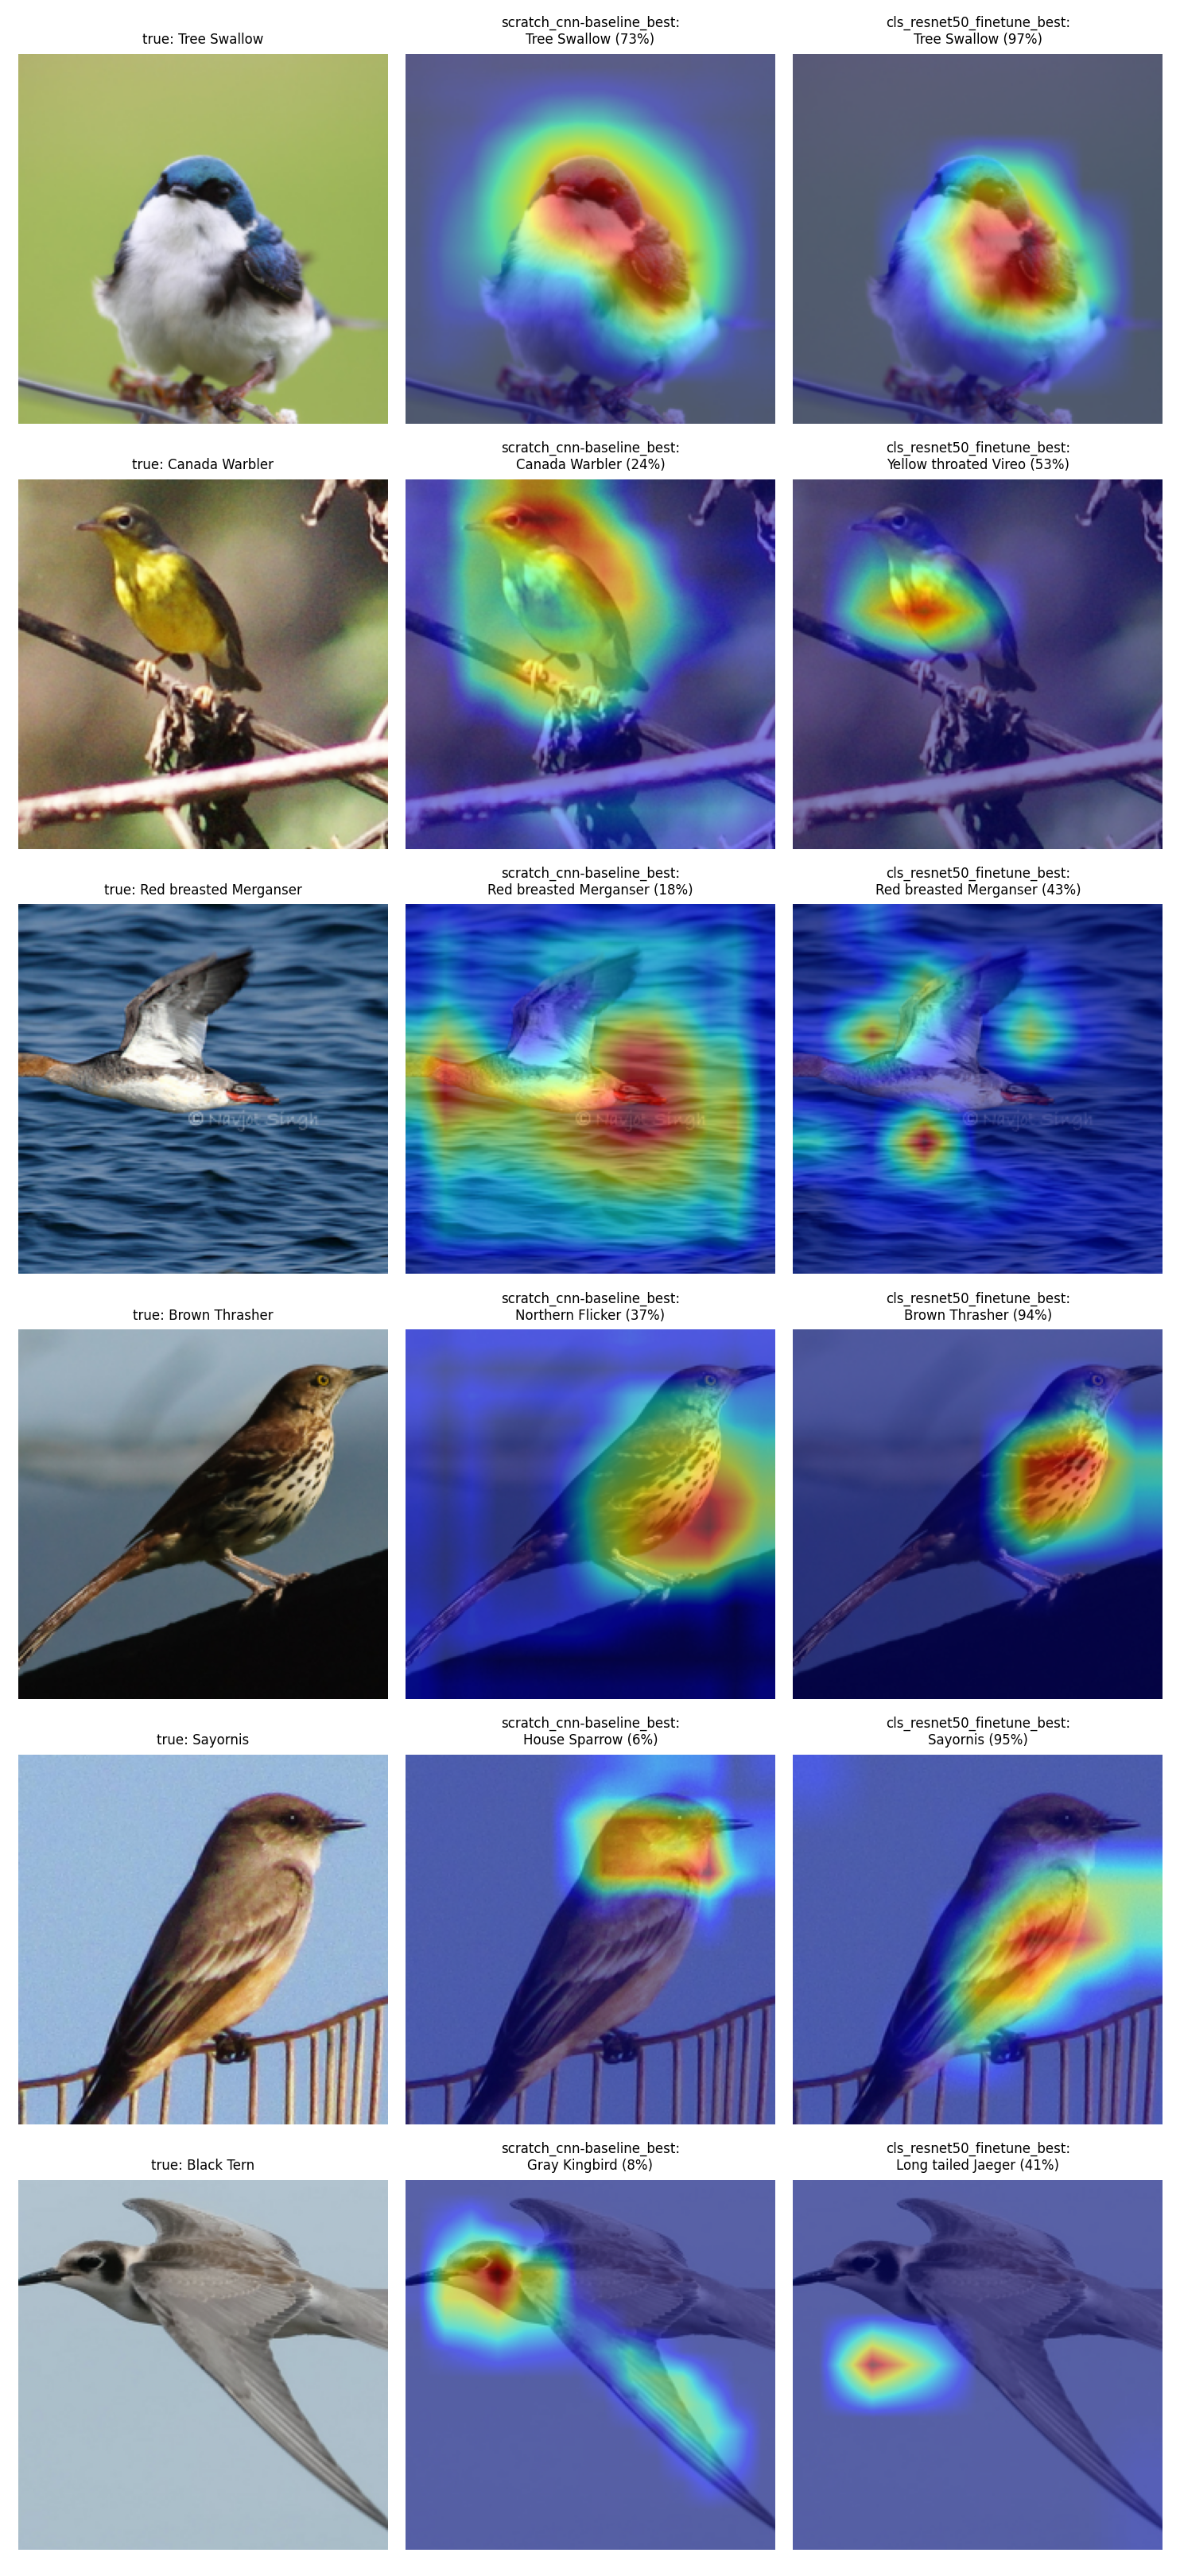
\includegraphics[height=0.62\textheight]{gradcam_scratch_vs_resnet50.png}
\caption{The same test images explained by both models. Left: input, middle: scratch CNN, right: fine-tuned ResNet-50.}
\label{fig:gradcam_compare}
\end{figure}

From Figures~\ref{fig:gradcam} and~\ref{fig:gradcam_compare} we noticed the following:
\begin{itemize}
  \item \textbf{ResNet-50, correct (92--100\% confidence):} the heatmap is on the body, breast and wing pattern of the bird, for example the stripes of the Black-and-white Warbler. The background stays cold.
  \item \textbf{ResNet-50, wrong (41--75\% confidence):} the confidence is clearly lower, so the model is ``aware'' that it is unsure. Most mistakes are lookalikes (Common Tern $\to$ Forster's Tern, Cliff Swallow $\to$ Barn Swallow). In a few cases the attention is off the bird, such as on the legs and perch of an Ovenbird. One Bank Swallow photographed from below in flight was called a Pomarine Jaeger, and the heatmap shows it was looking at the wing silhouette, which is the only thing visible against the sky.
  \item \textbf{Scratch CNN, wrong (4--37\% confidence):} it often looks at the \emph{background}. On an Elegant Tern the heat covers the water and the model predicts Horned Grebe, which is also a water bird. On a House Wren it looks at the sky. So with little data and no pretraining it learned shortcuts like ``water means water bird''.
  \item \textbf{Side by side:} on images where the scratch CNN fails (e.g.\ Brown Thrasher), ResNet-50 is right with about 95\% confidence and focuses on the spotted breast. However, Grad-CAM is not a proof that the model is right for the right reason: in one case ResNet-50 got a Red-breasted Merganser right with its attention scattered over the water.
\end{itemize}

% =====================================================
\section{Comparison with Published Results}

We compared our final model with published ResNet-50 results on the same official test split, using the same metric (top-1 accuracy) and the same kind of supervision (image labels only, no bounding boxes or part annotations).

\begin{table}[H]
\centering
\small
\begin{tabular}{l c c c}
\toprule
\textbf{Model} & \textbf{Input} & \textbf{Epochs} & \textbf{Test acc} \\
\midrule
\textbf{Ours, ResNet-50 fine-tuned} & 224 & 20 & \textbf{82.9\%} \\
ResNet-50, Li et al.~\cite{li2017dtram} & 224 & 90 & 81.5\% \\
ResNet-50, Li et al.~\cite{li2017dtram} / NTS-Net baseline~\cite{yang2018nts} & 448 & 90 & 84.5\% \\
ResNet-50, Xie et al.~\cite{xie2021cutthumbnail} & 448 & 95 & 85.3\% \\
NTS-Net, Yang et al.~\cite{yang2018nts} & 448 & -- & 87.5\% \\
\bottomrule
\end{tabular}
\caption{Our final model compared with published results on CUB-200-2011.}
\label{tab:benchmark}
\end{table}

At the same input size of 224\,px, our result matches the published ResNet-50 (81.5\%). Our small lead can be explained by the stronger ImageNet weights we use (\code{IMAGENET1K\_V2}, 80.9\% on ImageNet compared to about 76\% for the original weights), and also by noise, since the 95\% confidence interval on our test accuracy is about $\pm1$ point. The papers that report 84.5--85.3\% use 448\,px images, and Li et al.\ showed that going from 224 to 448 alone adds 3 points. This makes sense because the details that separate species only cover a few pixels at 224. We also train on 10\% fewer images (because of our validation set) and for fewer epochs, and we do not use any part-localization tricks like NTS-Net.

% =====================================================
\section{Limitations and Problems We Faced}

\begin{itemize}
  \item \textbf{Tuning did not help.} The 5-epoch trials were too short to rank the settings correctly, and the validation set is too small to tell apart settings within 1--2 points. Next time we would use longer trials or repeat each trial with different seeds.
  \item \textbf{The scratch CNN plateaued at 40\%} and uses background shortcuts. Stronger augmentation (e.g.\ CutMix), longer training or residual connections could help.
  \item \textbf{224\,px input limits the fine details.} Training at 448\,px is the main thing we would try next, although it costs about 4 times more compute.
  \item \textbf{Grad-CAM is coarse.} The maps are only $7\times7$ before resizing, so they show regions and not small parts like the eye ring.
  \item \textbf{No ``unknown'' option.} The classifier always picks one of the 200 species, even for a bird that is not in CUB.
\end{itemize}

We also ran into some engineering problems along the way. MLflow's default database path broke on Windows when the user folder name had a space in it, so we set the tracking URI ourselves. The \code{data/} rule in \code{.gitignore} accidentally hid \code{src/data/} as well. Two ResNet-50 runs had the same name and overwrote each other's checkpoint, so we started naming runs after their config file. Finally, we found out that the species list in the dataset is not in alphabetical order, so we had to save the class names in label order and never sort them.

% =====================================================
\section{Conclusion}

In this milestone we built a full pipeline for bird species classification on CUB-200-2011, from data analysis to explainability. The EDA helped us catch real issues such as train--test duplicates and noisy captions before training. Our results clearly show the value of transfer learning on a small fine-grained dataset: the accuracy went from 40.2\% for the scratch CNN to 64.3\% with a frozen ResNet-50 and 82.9\% after fine-tuning, which is in line with published results at the same resolution. Grad-CAM confirmed that the pretrained model looks at the bird while the scratch CNN often looks at the background. Our final model is the fine-tuned ResNet-50, and its encoder will be the backbone for the colorization and captioning tasks in Milestone 2.

% =====================================================
\begin{thebibliography}{99}
\small

\bibitem{wah2011cub}
C.~Wah, S.~Branson, P.~Welinder, P.~Perona, and S.~Belongie.
\newblock The Caltech-UCSD Birds-200-2011 dataset.
\newblock Technical Report CNS-TR-2011-001, California Institute of Technology, 2011.

\bibitem{reed2016}
S.~Reed, Z.~Akata, H.~Lee, and B.~Schiele.
\newblock Learning deep representations of fine-grained visual descriptions.
\newblock In \emph{CVPR}, 2016.

\bibitem{he2016resnet}
K.~He, X.~Zhang, S.~Ren, and J.~Sun.
\newblock Deep residual learning for image recognition.
\newblock In \emph{CVPR}, 2016.

\bibitem{selvaraju2017gradcam}
R.~R. Selvaraju, M.~Cogswell, A.~Das, R.~Vedantam, D.~Parikh, and D.~Batra.
\newblock Grad-CAM: Visual explanations from deep networks via gradient-based localization.
\newblock In \emph{ICCV}, 2017.

\bibitem{loshchilov2019adamw}
I.~Loshchilov and F.~Hutter.
\newblock Decoupled weight decay regularization.
\newblock In \emph{ICLR}, 2019.

\bibitem{loshchilov2017sgdr}
I.~Loshchilov and F.~Hutter.
\newblock SGDR: Stochastic gradient descent with warm restarts.
\newblock In \emph{ICLR}, 2017.

\bibitem{bergstra2012random}
J.~Bergstra and Y.~Bengio.
\newblock Random search for hyper-parameter optimization.
\newblock \emph{Journal of Machine Learning Research}, 13:281--305, 2012.

\bibitem{li2017dtram}
Z.~Li, Y.~Yang, X.~Liu, F.~Zhou, S.~Wen, and W.~Xu.
\newblock Dynamic computational time for visual attention.
\newblock arXiv:1703.10332, 2017.

\bibitem{yang2018nts}
Z.~Yang, T.~Luo, D.~Wang, Z.~Hu, J.~Gao, and L.~Wang.
\newblock Learning to navigate for fine-grained classification.
\newblock In \emph{ECCV}, 2018.

\bibitem{xie2021cutthumbnail}
T.~Xie, X.~Cheng, X.~Wang, M.~Liu, J.~Deng, T.~Zhou, and M.~Liu.
\newblock Cut-Thumbnail: A novel data augmentation for convolutional neural network.
\newblock In \emph{ACM Multimedia}, 2021.

\end{thebibliography}

\end{document}
